% Options for packages loaded elsewhere
\PassOptionsToPackage{unicode}{hyperref}
\PassOptionsToPackage{hyphens}{url}
\PassOptionsToPackage{dvipsnames,svgnames*,x11names*}{xcolor}
%
\documentclass[
]{article}
\usepackage{lmodern}
\usepackage{amssymb,amsmath}
\usepackage{ifxetex,ifluatex}
\ifnum 0\ifxetex 1\fi\ifluatex 1\fi=0 % if pdftex
  \usepackage[T1]{fontenc}
  \usepackage[utf8]{inputenc}
  \usepackage{textcomp} % provide euro and other symbols
\else % if luatex or xetex
  \usepackage{unicode-math}
  \defaultfontfeatures{Scale=MatchLowercase}
  \defaultfontfeatures[\rmfamily]{Ligatures=TeX,Scale=1}
\fi
% Use upquote if available, for straight quotes in verbatim environments
\IfFileExists{upquote.sty}{\usepackage{upquote}}{}
\IfFileExists{microtype.sty}{% use microtype if available
  \usepackage[]{microtype}
  \UseMicrotypeSet[protrusion]{basicmath} % disable protrusion for tt fonts
}{}
\makeatletter
\@ifundefined{KOMAClassName}{% if non-KOMA class
  \IfFileExists{parskip.sty}{%
    \usepackage{parskip}
  }{% else
    \setlength{\parindent}{0pt}
    \setlength{\parskip}{6pt plus 2pt minus 1pt}}
}{% if KOMA class
  \KOMAoptions{parskip=half}}
\makeatother
\usepackage{xcolor}
\IfFileExists{xurl.sty}{\usepackage{xurl}}{} % add URL line breaks if available
\IfFileExists{bookmark.sty}{\usepackage{bookmark}}{\usepackage{hyperref}}
\hypersetup{
  colorlinks=true,
  linkcolor=blue,
  filecolor=Maroon,
  citecolor=Blue,
  urlcolor=Blue,
  pdfcreator={LaTeX via pandoc}}
\urlstyle{same} % disable monospaced font for URLs
\usepackage{longtable,booktabs}
% Correct order of tables after \paragraph or \subparagraph
\usepackage{etoolbox}
\makeatletter
\patchcmd\longtable{\par}{\if@noskipsec\mbox{}\fi\par}{}{}
\makeatother
% Allow footnotes in longtable head/foot
\IfFileExists{footnotehyper.sty}{\usepackage{footnotehyper}}{\usepackage{footnote}}
\makesavenoteenv{longtable}
\usepackage{graphicx}
\makeatletter
\def\maxwidth{\ifdim\Gin@nat@width>\linewidth\linewidth\else\Gin@nat@width\fi}
\def\maxheight{\ifdim\Gin@nat@height>\textheight\textheight\else\Gin@nat@height\fi}
\makeatother
% Scale images if necessary, so that they will not overflow the page
% margins by default, and it is still possible to overwrite the defaults
% using explicit options in \includegraphics[width, height, ...]{}
\setkeys{Gin}{width=\maxwidth,height=\maxheight,keepaspectratio}
% Set default figure placement to htbp
\makeatletter
\def\fps@figure{htbp}
\makeatother
\setlength{\emergencystretch}{3em} % prevent overfull lines
\providecommand{\tightlist}{%
  \setlength{\itemsep}{0pt}\setlength{\parskip}{0pt}}
\setcounter{secnumdepth}{5}

%% pandoc-tablenos: required package
\usepackage{cleveref}

%% pandoc-eqnos: disable brackets around cleveref numbers
\creflabelformat{equation}{#2#1#3}
\ifluatex
  \usepackage{selnolig}  % disable illegal ligatures
\fi

\author{}
\date{}

\begin{document}

\newcommand{\df}[1]{\frac{\partial}{\partial #1}}

\hypertarget{principal-component-analysis}{%
\section{Principal Component
Analysis}\label{principal-component-analysis}}

\hypertarget{introduction}{%
\subsection{Introduction}\label{introduction}}

Suppose that, as usual, we begin with a collection of measurements of
different features for a group of samples. Some of these measurements
will tell us quite a bit about the difference among our samples, while
others may contain relatively little information. For example, if we are
analyzing the effect of a certain weight loss regimen on a group of
people, the age and weight of the subjects may have a great deal of
influence on how successful the regimen is, while their blood pressure
might not. One way to help identify which features are more significant
is to ask whether or not the feature varies a lot among the different
samples. If nearly all the measurements of a feature are the same, it
can't have much power in distinguishing the samples, while if the
measurements vary a great deal then that feature has a chance to contain
useful information.

In this section we will discuss a way to measure the variability of
measurements and then introduce principal component analysis (PCA). PCA
is a method for finding which linear combinations of measurements have
the greatest variability and therefore might contain the most
information. It also allows us to identify combinations of measurements
that don't vary much at all. Combining this information, we can
sometimes replace our original system of features with a smaller set
that still captures most of the interesting information in our data, and
thereby find hidden characteristics of the data and simplify our
analysis a great deal.

\hypertarget{variance-and-covariance}{%
\subsection{Variance and Covariance}\label{variance-and-covariance}}

\hypertarget{variance}{%
\subsubsection{Variance}\label{variance}}

Suppose that we have a collection of measurements \((x_1,\ldots, x_n)\)
of a particular feature \(X\). For example, \(x_i\) might be the initial
weight of the \(ith\) participant in our weight loss study. The mean of
the values \((x_1,\ldots, x_n)\) is

\[
\mu_{X} = \frac{1}{n}\sum_{i=1}^{n} x_{i}.
\]

The simplest measure of the variability of the data is called its
\emph{variance.}

\textbf{Definition:} The (sample) variance of the data
\(x_1,\ldots, x_n\) is

\begin{equation}
\sigma_{X}^2 = \frac{1}{n}\sum_{i=1}^{n} \left(x_{i}-\mu_{X}\right)^2 = \frac{1}{n}\left(\sum_{i=1}^{n} x_{i}^2\right)- \mu_{X}^2
\label{eq:variance}\end{equation}

The square root of the variance is called the \emph{standard deviation.}

As we see from the formula, the variance is a measure of how `spread
out' the data is from the mean.

Recall that in our discussion of linear regression we thought of our set
of measurements \(x_1,\ldots, x_n\) as a vector -- it's one of the
columns of our data matrix. From that point of view, the variance has a
geometric interpretation -- it is \(\frac{1}{N}\) times the square of
the distance from the point \(X=(x_1,\ldots, x_n)\) to the point
\(\mu_{X}(1,1,\ldots,1)=\mu_{X}E\):

\begin{equation}
\sigma_{X}^2 = \frac{1}{n}(X-\mu_{X}E)\cdot(X-\mu_{X}E)  = \frac{1}{n}\|X-\mu_{X}E\|^2.
\label{eq:variancedot}\end{equation}

\hypertarget{covariance}{%
\subsubsection{Covariance}\label{covariance}}

The variance measures the dispersion of measures of a single feature.
Often, we have measurements of multiple features and we might want to
know something about how two features are related. The \emph{covariance}
is a measure of whether two features tend to be related, in the sense
that when one increases, the other one increases; or when one increases,
the other one decreases.

\textbf{Definition:} Given measurements \((x_1,\ldots, x_n)\) and
\((y_1,\ldots, y_n)\) of two features \(X\) and \(Y\), the covariance of
\(X\) and \(Y\) is

\begin{equation}
\sigma_{XY} = \frac{1}{N}\sum_{i=1}^{N} x_iy_i
\label{eq:covariancedot}\end{equation}

There is a nice geometric interpretation of this, as well, in terms of
the dot product. If \(X=(x_1,\ldots, x_n)\) and \(Y=(y_1\ldots,y_n)\)
then

\[
\sigma_{XY} = \frac{1}{N} ((X-\mu_{X}E)\cdot (Y-\mu_{Y}E)).
\]

From this point of view, we can see that \(\sigma_{XY}\) is positive if
the \(X-\mu_{X}E\) and \(Y-\mu_{Y}E\) vectors ``point roughly in the
same direction'' and its negative if they ``point roughly in the
opposite direction.''

\hypertarget{correlation}{%
\subsubsection{Correlation}\label{correlation}}

One problem with interpreting the variance and covariance is that we
don't have a scale -- for example, if \(\sigma_{XY}\) is large and
positive, then we'd like to say that \(X\) and \(Y\) are closely
related, but it could be just that the entries of \(X-\mu_{X}E\) and
\(Y-\mu_{Y}E\) are large. Here, though, we can really take advantage of
the geometric interpretation. Recall that the dot product of two vectors
satisfies the formula

\[
a \cdot b = \|a\|\|b\|\cos(\theta)
\]

where \(\theta\) is the angle between \(a\) and \(b\). So

\[
\cos(\theta) = \frac{a\cdot b}{\|a\|\|b\|}.
\]

Let's apply this to the variance and covariance, by noticing that

\[
\frac{(X-\mu_{X}E)\cdot (Y-\mu_{Y}E)}{\|(X-\mu_{X}E)\|\|(Y-\mu_{Y}E)\|} = \frac{\sigma_{XY}}{\sigma_{XX}\sigma_{YY}}
\]

so the quantity

\begin{equation}
r_{XY} = \frac{\sigma_{XY}}{\sigma_{X}\sigma_{Y}}
\label{eq:rxy}\end{equation}

measures the cosine of the angle between the vectors \(X-\mu_{X}E\) and
\(Y-\mu_{Y}E\).

\textbf{Definition:} The quantity \(r_{XY}\) defined in \cref{eq:rxy} is
called the (sample) \emph{correlation coefficient} between \(X\) and
\(Y\). We have \(0\le |r_{XY}|\le 1\) with \(r_{XY}=\pm 1\) if and only
if the two vectors \(X-\mu_{X}\) and \(Y-\mu_{Y}\) are collinear in
\(\mathbf{R}^{n}\).

\Cref{fig:corrfig} illustrates data with different values of the
correlation coefficient.

\begin{figure}
\hypertarget{fig:corrfig}{%
\centering
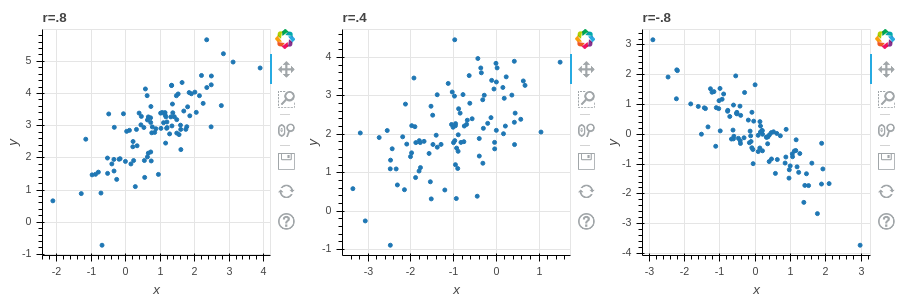
\includegraphics[width=0.5\textwidth,height=\textheight]{../img/correlation.png}
\caption{Correlation}\label{fig:corrfig}
}
\end{figure}

\hypertarget{sec:covarmat}{%
\subsubsection{The covariance matrix}\label{sec:covarmat}}

In a typical situation we have many features for each of our (many)
samples, that we organize into a data matrix \(X\). To recall, each
column of \(X\) corresponds to a feature that we measure, and each row
corresponds to a sample. For example, each row of our matrix might
correspond to a person enrolled in a study, and the columns correspond
to height (cm), weight (kg), systolic blood pressure, and age (in
years):

\begin{longtable}[]{@{}lrrrr@{}}
\caption{A sample data matrix \(X\) \label{tbl:data}}\tabularnewline
\toprule
sample & Ht & Wgt & Bp & Age\tabularnewline
\midrule
\endfirsthead
\toprule
sample & Ht & Wgt & Bp & Age\tabularnewline
\midrule
\endhead
A & 180 & 75 & 110 & 35\tabularnewline
B & 193 & 80 & 130 & 40\tabularnewline
\ldots{} & \ldots{} & \ldots{} & \ldots{} & \ldots{}\tabularnewline
U & 150 & 92 & 105 & 55\tabularnewline
\bottomrule
\end{longtable}

If we have multiple features, as in this example, we might be interested
in the variance of each feature and all of their mutual covariances.
This ``package'' of information can be obtained ``all at once'' by
taking advantage of some matrix algebra.

\textbf{Definition:} Let \(X\) be a \(k\times N\) data matrix, where the
\(N\) columns of \(X\) correspond to different features and the \(k\)
rows to different samples. Let \(X_{0}\) be the centered version of this
data matrix, obtained by subtracting the mean \(\mu_{i}\) of column
\(i\) from all the entries \(x_{si}\) in that column. Then the
\(N\times N\) symmetric matrix

\[
D_{0} = \frac{1}{N}X_{0}^{\intercal}X_{0}
\]

is called the (sample) covariance matrix for the data.

\textbf{Proposition:} The diagonal entries \(d_{ii}\) of \(D_{0}\) are
the variances of the columns of \(X\):

\[
d_{ii} = \sigma_{i}^2 = \frac{1}{N}\sum_{s=1}^{k}(x_{si}-\mu_i)^2
\]

and the off-diagonal entries \(d_{ij} = d_{ji}\) are the covariances of
the \(i^{th}\) and \(j^{th}\) columns of \(X\):

\[
d_{ij} = \sigma_{ij} = \frac{1}{N}\sum_{s=1}^{k}(x_{si}-\mu_{i})(x_{sj}-\mu_{j})
\]

The sum of the diagonal entries, the trace of \(D_{0}\) is the
\textbf{total} variance of the data.

\textbf{Proof:} This follows from the definitions, but it's worth
checking the details, which we leave as an exercise.

\hypertarget{sec:visualizecovar}{%
\subsubsection{Visualizing the covariance
matrix}\label{sec:visualizecovar}}

If the number of features in the data is not too large, a density matrix
plot provides a tool for visualizing the covariance matrix of the data.
A density matrix plot is an \(N\times N\) grid of plots (where \(N\) is
the number of features). The entry with \((i,j)\) coordinates in the
grid is a scatter plot of the \(i^{th}\) feature against the \(j^{th}\)
one if \(i\not=j\), and is a histogram of the \(i^{th}\) variable if
\(i=j\).

\Cref{fig:density0} is an example of a density matrix plot for a dataset
with \(50\) samples and \(2\) features. This data has been centered, so
it can be represented in a \(50\times 2\) data matrix \(X_{0}\). The
upper left and lower right graphs are scatter plots of the two columns,
while the lower left and upper right are the histograms of the columns.

\begin{figure}
\hypertarget{fig:density0}{%
\centering
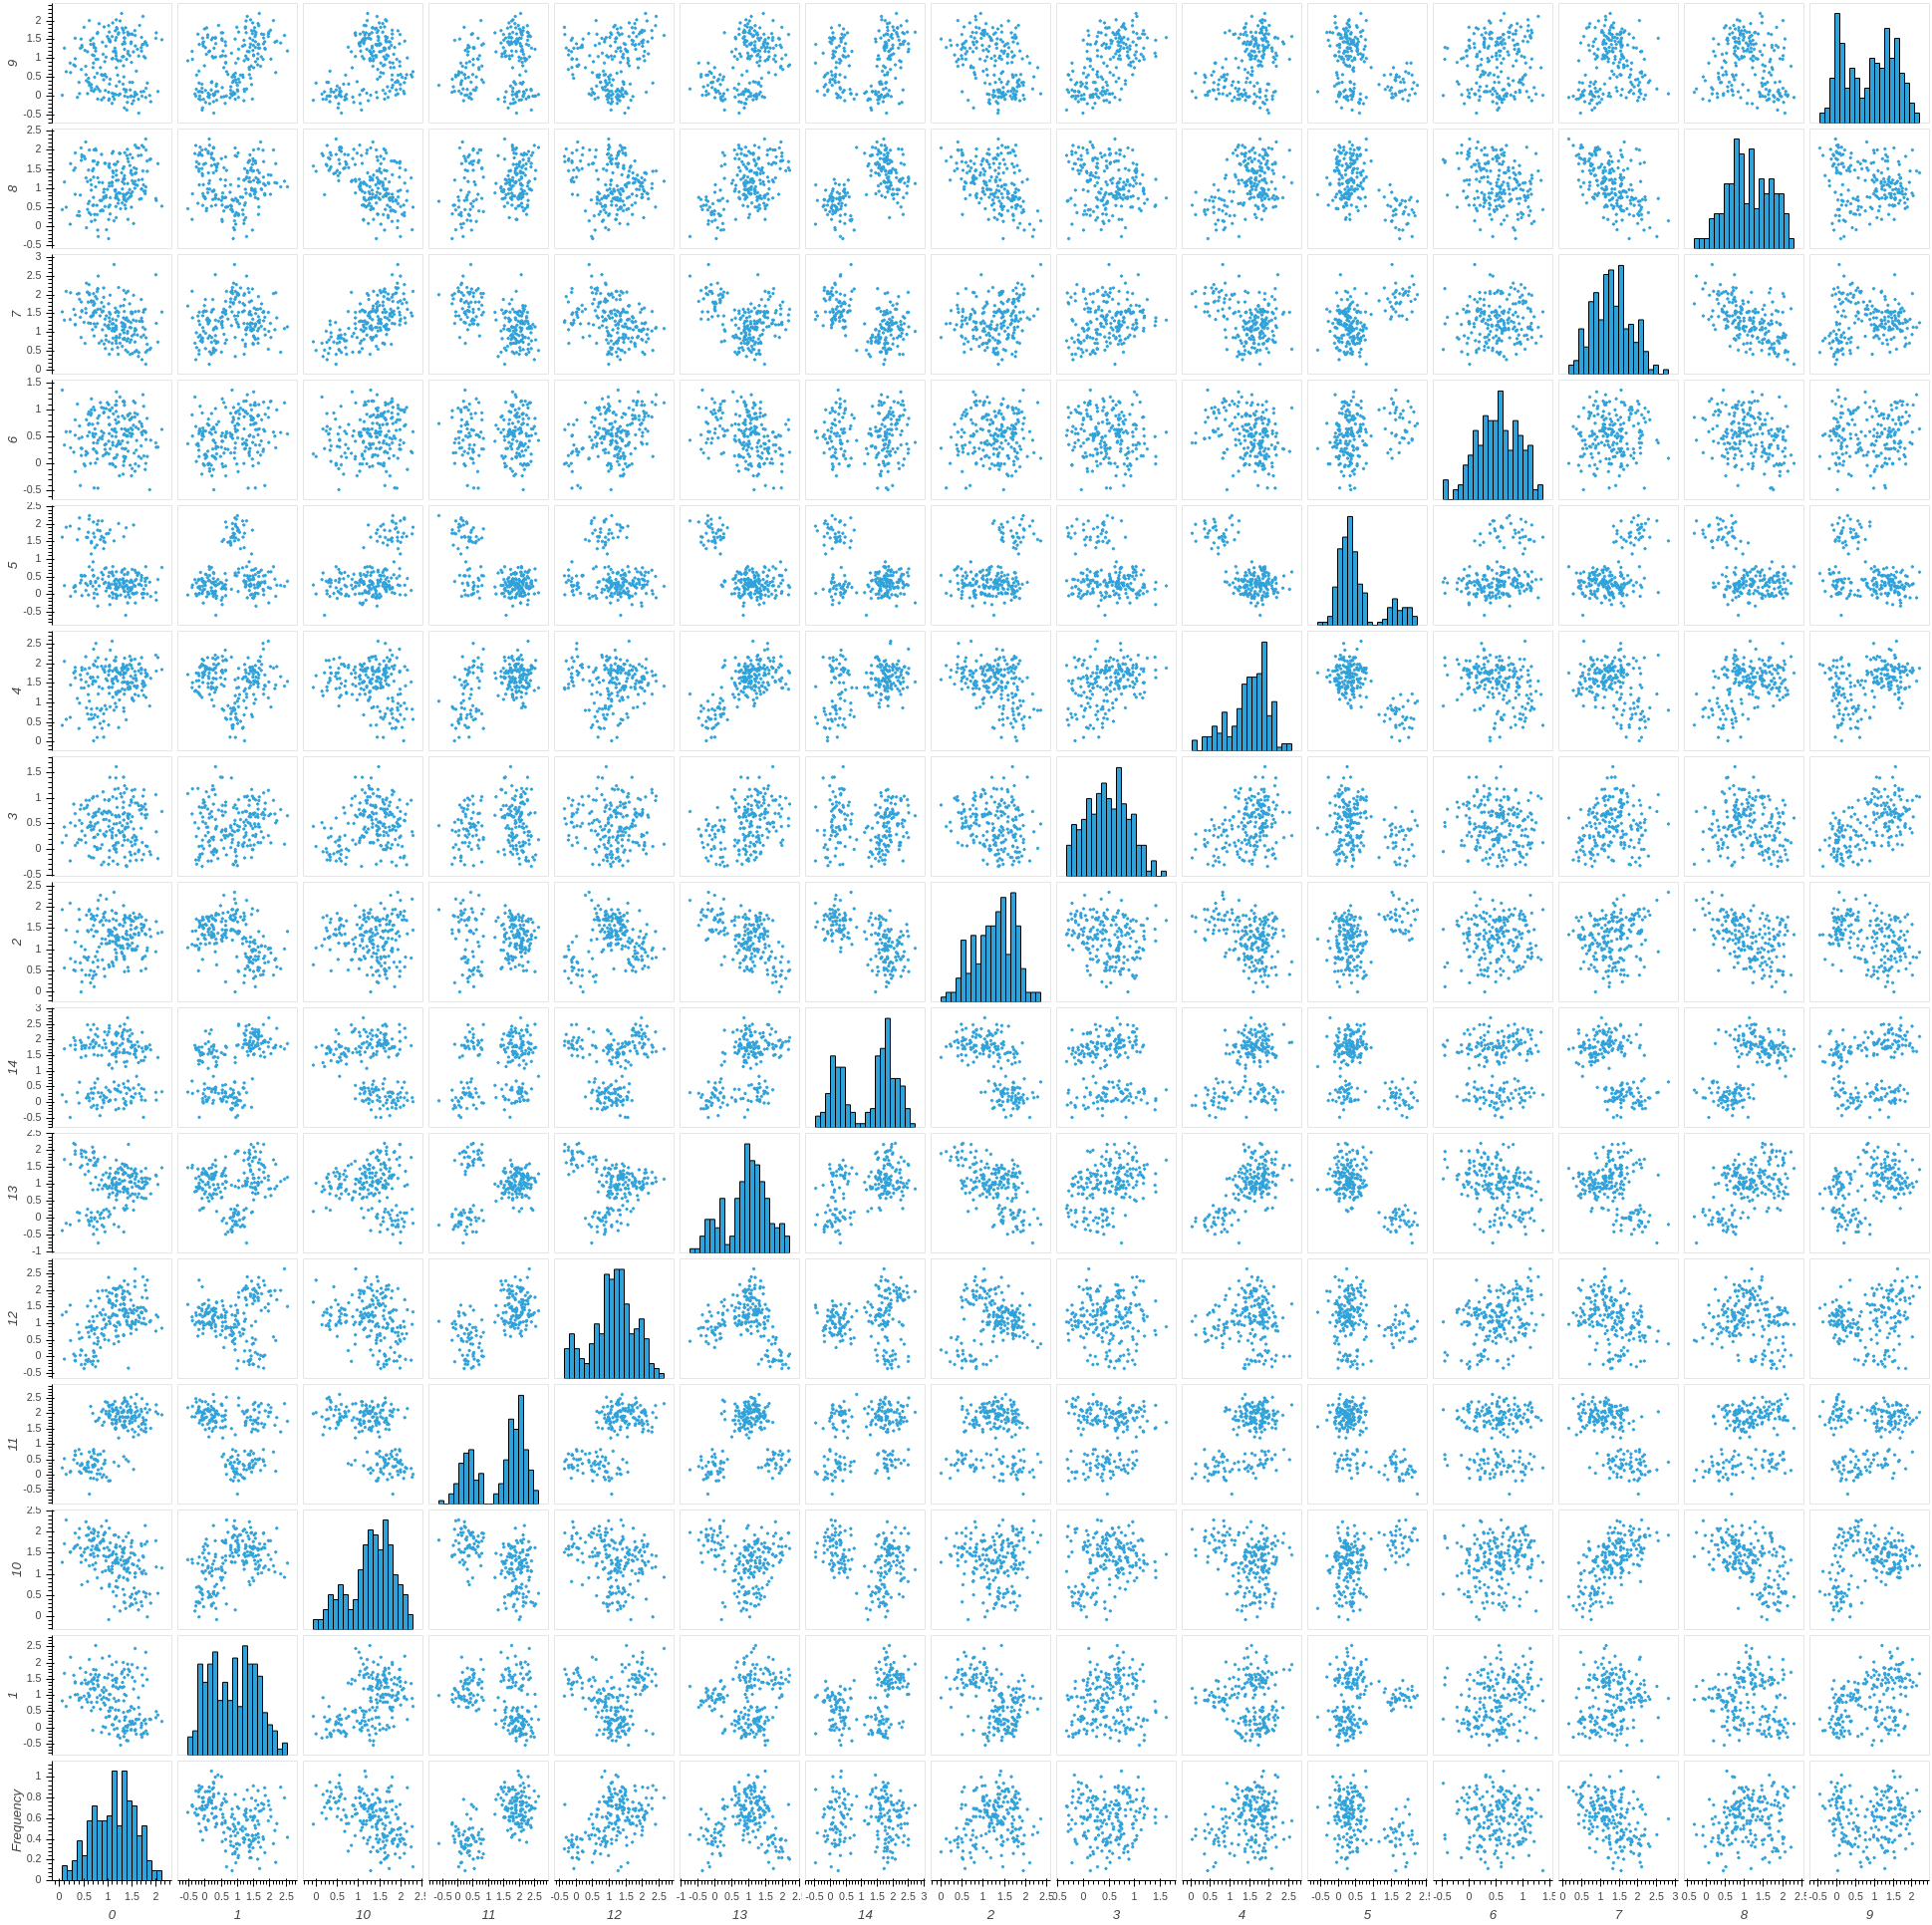
\includegraphics[width=0.5\textwidth,height=\textheight]{../img/density.png}
\caption{Density Matrix Plot}\label{fig:density0}
}
\end{figure}

\hypertarget{linear-combinations-of-features-scores}{%
\subsubsection{Linear Combinations of Features
(Scores)}\label{linear-combinations-of-features-scores}}

Sometimes useful information about our data can be revealed if we
combine different measurements together to obtain a ``hybrid'' measure
that captures something interesting. For example, in the Auto MPG
dataset that we studied in the section on Linear Regression, we looked
at the influence of both vehicle weight \(w\) and engine displacement
\(e\) on gas mileage; perhaps their is some value in considering a
hybrid ``score'' defined as \[
S = aw + be
\] for some constants \(a\) and \(b\) -- maybe by choosing a good
combination we could find a better predictor of gas mileage than using
one or the other of the features individually.

As another example, suppose we are interested in the impact of the
nutritional content of food on weight gain in a study. We know that both
calorie content and the level dietary fiber contribute to the weight
gain of participants eating this particular food; maybe there is some
kind of combined ``calorie/fiber'' score we could introduce that
captures the impact of that food better.

\textbf{Definition:} Let \(X_{0}\) be a (centered) \(k\times N\) data
matrix giving information about \(N\) features for each of \(k\)
samples. A linear synthetic feature, or a linear score, is a linear
combination of the \(N\) features. The linear score is defined by
constants \(a_{1},\ldots, a_{n}\) so that If \(y_{1},\ldots, y_{N}\) are
the values of the features for a particular sample, then the linear
score for that sample is

\[
S = a_{1}y_{1}+a_{2}y_{2}+\cdots+a_{N}y_{N}
\]

\textbf{Lemma:} The values of the linear score for each of the \(k\)
samples can be calculated as

\begin{equation}
\left[\begin{matrix} S_{1} \\ \vdots \\ S_{k}\\ \end{matrix}\right] =
X_{0}\left[
\begin{matrix} a_{1} \\ \vdots \\ a_{N}\end{matrix}\right].
\label{eq:linearscore}\end{equation}

\textbf{Proof:} Multiplying a matrix by a column vector computes a
linear combination of the columns -- that's what this lemma says.
Exercise 3 asks you to write out the indices and make sure you believe
this.

\hypertarget{mean-and-variance-of-scores}{%
\subsubsection{Mean and variance of
scores}\label{mean-and-variance-of-scores}}

When we combine features to make a hybrid score, we assume that the
features were centered to begin with, so that each features has mean
zero. As a result, the mean of the hybrid features is again zero.

\textbf{Lemma:} A linear combination of features with mean zero again
has mean zero.

\textbf{Proof:} Let \(S_{i}\) be the score for the \(i^{th}\) sample, so
\[
S_{i} = \sum_{j=1}^{N} x_{ij}a_{j}.
\] where \(X_{0}\) has entries \(x_{ij}\). Then the mean value of the
score is \[
\mu_{S} = \frac{1}{k}\sum_{i=1}^{k} S_{i} = \frac{1}{k}\sum_{i=1}^{k}\sum_{j=1}^{N} x_{ij}a_{j}.
\] Reversing the order of the sum yields \[
\mu_{S} = \frac{1}{k}\sum_{j=1}^{N}\sum_{i=1}^{k} x_{ij}a_{j} = \sum_{j=1}^{N} a_{j}\frac{1}{k}(\sum_{i=1}^{k} x_{ij})=
\sum_{j=1}^{N}a_{j}\mu_{j}=0
\] where \(\mu_{j}=0\) is the mean of the \(j^{th}\) feature (column) of
\(X_{0}\).

The variance is more interesting, and gives us an opportunity to put the
covariance matrix to work. Remember from \ref{eq:variancedot} that,
since a score \(S\) has mean zero, it's variance is
\(\sigma_{S}^2=S\cdot S\) -- where here the score \(S\) is represented
by the column vector with entries \(S_{1},\ldots S_{k}\) as in
\cref{eq:linearscore}.

\textbf{Lemma:} The variance of the score \(S\) with weights
\(a_1,\ldots a_N\) is \begin{equation}
\sigma_{S}^2 = a^{\intercal}D_{0}a = \left[\begin{matrix}a_{1} & \cdots & a_{N}\end{matrix}\right]D_{0}
\left[\begin{matrix} a_{1} \\ \vdots \\ a_{N}\end{matrix}\right]
\label{eq:ada}\end{equation} More generally, if \(S_{1}\) and \(S_{2}\)
are scores with weights \(a_1,\ldots, a_N\) and \(b_1,\ldots, b_N\)
respectively, then the covariance \(\sigma_{S_{1}S_{2}}\) is \[
\sigma_{S_{1}S_{2}} = a^{\intercal}D_{0}b.
\]

\textbf{Proof:} From \cref{eq:variancedot} and \ref{eq:linearscore} we
know that \[
\sigma_{S}^2 = S\cdot S
\] and \[
S = X_{0}a.
\] Since \(S\cdot S = \frac{1}{N}S^{\intercal}S\), this gives us \[
\sigma_{S}^2 = \frac{1}{N}(X_{0}a)^{\intercal}(X_{0}a) = \frac{1}{N}a^{\intercal}X_{0}^{\intercal}X_{0}a = a^{\intercal}D_{0}a
\] as claimed.

For the covariance, use a similar argument with \cref{eq:covariancedot}
and \cref{eq:linearscore}. writing
\(\sigma_{S_{1}S_{2}}=\frac{1}{N}S_{1}\cdot S_{2}\) and the fact that
\(S_{1}\) and \(S_{2}\) can be written as \(X_{0}a\) and \(X_{0}b\).

The point of this lemma is that the covariance matrix contains not just
the variances and covariances of the original features, but also enough
information to construct the variances and covariances for \emph{any
linear combination of features.}

In the next section we will see how to exploit this idea to reveal
hidden structure in our data.

\hypertarget{geometry-of-scores}{%
\subsubsection{Geometry of Scores}\label{geometry-of-scores}}

Let's return to the dataset that we looked at in
\cref{sec:visualizecovar}. We simplify the density matrix plot in
\cref{fig:pcasimfig}, which shows one of the scatter plots and the two
histograms.

The scatter plot shows that the data points are arranged in a more or
less elliptical cloud oriented at an angle to the \(xy\)-axes which
represent the two given features. The two individual histograms show the
distribution of the two features -- each has mean zero, with the
\(x\)-features distributed between \(-2\) and \(2\) and the \(y\)
feature between \(-4\) and \(4\). Looking just at the two features
individually, meaning only at the two histograms, we can't see the
overall elliptical structure.

\begin{figure}
\hypertarget{fig:pcasimfig}{%
\centering
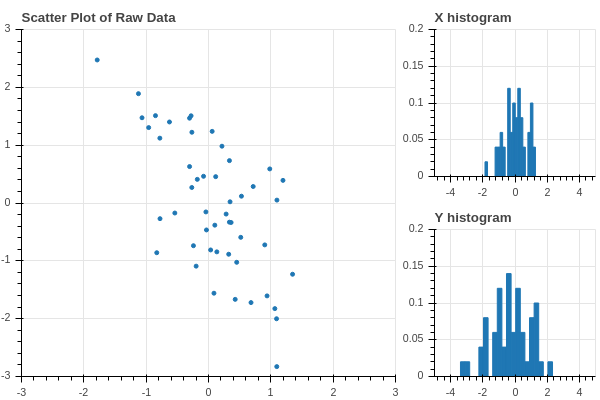
\includegraphics[width=0.5\textwidth,height=\textheight]{../img/PCAsimulated-1.png}
\caption{Simulated Data with Two Features}\label{fig:pcasimfig}
}
\end{figure}

How can we get a better grip on our data in this situation? We can try
to find a ``direction'' in our data that better illuminates the
variation of the data. For example, suppose that we pick a unit vector
at the origin pointing in a particular direction in our data. See
\cref{fig:pcasimfig-1}.

\begin{figure}
\hypertarget{fig:pcasimfig-1}{%
\centering
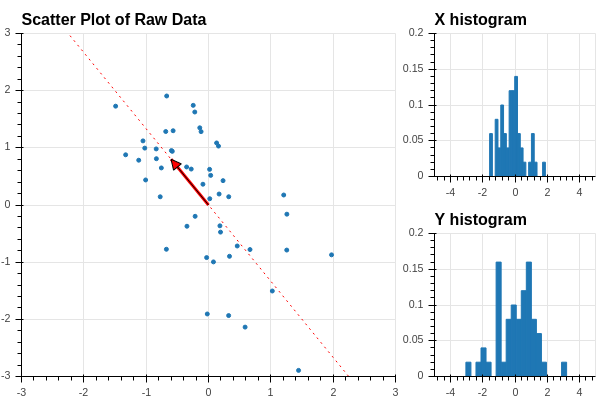
\includegraphics[width=0.5\textwidth,height=\textheight]{../img/PCAsimulated-2.png}
\caption{A direction in the data}\label{fig:pcasimfig-1}
}
\end{figure}

Now we can orthogonally project the datapoints onto the line defined by
this vector, as shown in \cref{fig:pcasimfig-2}.

\begin{figure}
\hypertarget{fig:pcasimfig-2}{%
\centering
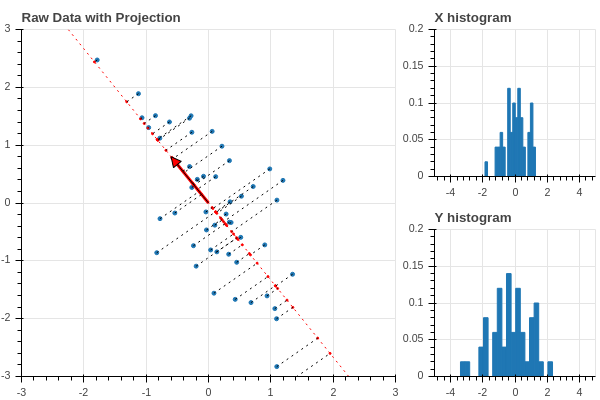
\includegraphics[width=0.5\textwidth,height=\textheight]{../img/PCAsimulated-3.png}
\caption{Projecting the datapoints}\label{fig:pcasimfig-2}
}
\end{figure}

Recall that if the unit vector is defined by coordinates
\(u=[u_0,u_1]\), then the orthogonal projection of the point \(x\) with
coordinates \((x_0,x_1)\) is \((x\cdot u)u\). Now \[
x\cdot u = u_0 x_0 + u_1 x_1
\] so the coordinates of the points along the line defined by \(u\) are
the values of the score \(Z\) defined by \(u=[u_0,u_1]\). Using our work
in the previous section, we see that we can find all of these
coordinates by matrix multiplication: \[
Z = X_0 u
\] where \(X_0\) is our data matrix. Now let's add a histogram of the
values of \(Z\) to our picture:

\begin{figure}
\hypertarget{fig:pcasimfig-3}{%
\centering
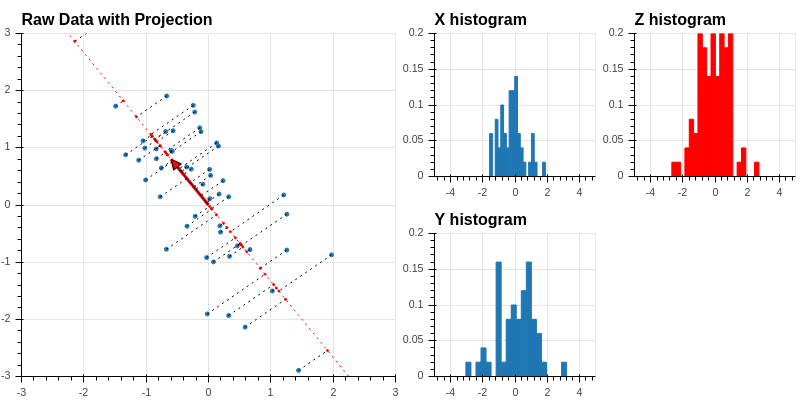
\includegraphics[width=0.5\textwidth,height=\textheight]{../img/PCAsimulated-4.png}
\caption{Distribution of Z}\label{fig:pcasimfig-3}
}
\end{figure}

This histogram shows the distribution of the values of \(Z\) along the
tilted line defined by the unit vector \(u\).

Finally, using our work on the covariance matrix, we see that the
variance of \(Z\) is given by \[
\sigma_{Z}^2 = \frac{1}{50}u^{\intercal}X_{0}^{\intercal}X_{0}u = u^{\intercal}D_{0}u
\] where \(D_{0}\) is the covariance matrix of the data \(X_{0}\).

\textbf{Lemma:} Let \(X_{0}\) be a \(k\times N\) centered data matrix,
and let \(D_{0}=\frac{1}{N}X_{0}^{\intercal}X_{0}\) be the associated
covariance matrix. Let \(u\) be a unit vector in ``feature space''
\(\mathbf{R}^{N}\). Then the score \(S=X_{0}u\) can be interpreted as
the coordinates of the points of \(X_{0}\) projected onto the line
generated by \(u\). The variance is \[
\sigma^{2}_{S} = u^{\intercal}D_{0}u = \sum_{i=1}^{k} s_{i}^2
\] where \(s_{i} = X_{0}[i,:]u\) is the dot product of the \(i^{th}\)
row \(X_{0}[i,:]\) with \(u\). It measures the variability in the data
``in the direction of the unit vector \(u\)''.

\hypertarget{principal-components}{%
\subsection{Principal Components}\label{principal-components}}

\hypertarget{change-of-variance-with-direction}{%
\subsubsection{Change of variance with
direction}\label{change-of-variance-with-direction}}

As we've seen in the previous section, if we choose a unit vector \(u\)
in the feature space and find the projection \(X_{0}u\) of our data onto
the line through \(u\), we get a ``score'' that we can use to measure
the variance of the data in the direction of \(u\). What happens as we
vary \(u\)?

To study this question, let's continue with our simulated data from the
previous section, and introduce a unit vector \[
u(\theta) = \left[\begin{matrix} \cos(\theta) & \sin(\theta)\end{matrix}\right].
\] This is in fact a unit vector, since
\(\sin^2(\theta)+\cos^2(\theta)=1\), and it is oriented at an angle
\(\theta\) from the \(x\)-axis.

The variance of the data in the direction of \(u(\theta)\) is given by
\[
\sigma_{\theta}^2 = u(\theta)^{\intercal}D_{0}u(\theta).
\]

A plot of this function for the data we have been considering is in
\cref{fig:pcatheta}. As you can see, the variance goes through two full
periods with the angle, and it reaches a maximum and minimum value at
intervals of \(\pi/2\) -- so the two angles where the variance are
maximum and minimum are orthogonal to one another.

\begin{figure}
\hypertarget{fig:pcatheta}{%
\centering
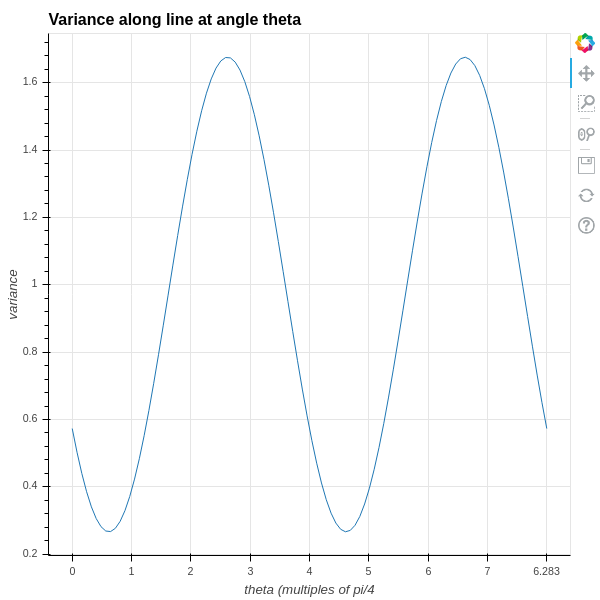
\includegraphics[width=0.25\textwidth,height=\textheight]{../img/PCAtheta.png}
\caption{Change of variance with angle theta}\label{fig:pcatheta}
}
\end{figure}

The two directions where the variance is maximum and minimum are drawn
on the original data scatter plot in \cref{fig:pcaprincipal} .

\begin{figure}
\hypertarget{fig:pcaprincipal}{%
\centering
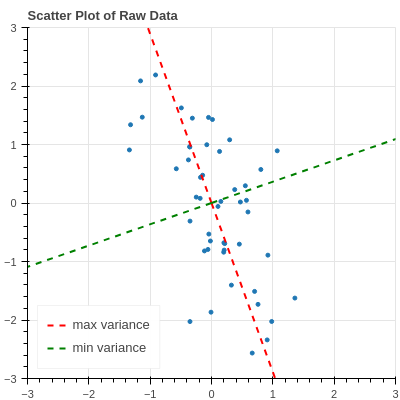
\includegraphics[width=0.25\textwidth,height=\textheight]{../img/PCAprincipal.png}
\caption{Data with principal directions}\label{fig:pcaprincipal}
}
\end{figure}

Let's try to understand why this is happening.

\hypertarget{sec:extremalvariance}{%
\subsubsection{Directions of extremal
variance}\label{sec:extremalvariance}}

Given our centered, \(k\times N\) data matrix \(X_{0}\), with its
associated covariance matrix
\(D_{0}=\frac{1}{N}X_{0}^{\intercal}X_{0}\), we would like to find unit
vectors \(u\) in \(\mathbf{R}^{N}\) so that \[
\sigma_{u}^{2} = u^{\intercal}D_{0}u
\] reaches its maximum and its minimum. Here \(\sigma_{u}^2\) is the
variance of the ``linear score'' \(X_{0}u\) and it represents how
dispersed the data is in the ``u direction'' in \(\mathbf{R}^{N}\).

In this problem, remember that the coordinates of
\(u=(u_1,\ldots, u_{N})\) are the variables and the symmetric matrix
\(D_{0}\) is given. As usual, we to find the maximum and minimum values
of \(\sigma_{u}^{2}\), we should look at the partial derivatives of
\(\sigma_{u}^{2}\) with respect to the variables \(u_{i}\) and set them
to zero. Here, however, there is a catch -- we want to restrict \(u\) to
being a unit vector, with \(u\cdot u =\sum u_{i}^2=1\).

So this is a \emph{constrained optimization problem}:

\begin{itemize}
\tightlist
\item
  Find extreme values of the function \[
  \sigma_{u}^{2} = u^{\intercal}D_{0}u
  \]
\item
  Subject to the constraint \(\|u\|^2 = u\cdot u=1\) (or
  \(u\cdot u-1=0\))
\end{itemize}

We will use the technique of \emph{Lagrange Multipliers} to solve such a
problem.

To apply this method, we introduce the function

\begin{equation}
S(u, \lambda) = u^{\intercal}D_{0}u - \lambda(u\cdot u -1)
\label{eq:lagrange}\end{equation}

Then we compute the gradient

\begin{equation}
\nabla S = \left[\begin{matrix} \frac{\partial S}{\partial u_{1}} \\ \vdots \\ \frac{\partial S}{\partial u_{N}} \\ \frac{\partial S}{\partial \lambda}\end{matrix}\right]
\label{eq:lagrangegradient}\end{equation}

and solve the system of equations \(\nabla S=0\). Here we have written
the gradient as a column vector for reasons that will become clearer
shortly.

Computing all of these partial derivatives looks messy, but actually if
we take advantage of matrix algebra it's not too bad. The following two
lemmas explain how to do this.

\textbf{Lemma}: Let \(M\) be a \(k\times N\) matrix with constant
coefficients and let \(u\) be a \(N\times 1\) column vector whose
entries are \(u_1,\ldots u_{N}\). The function \(F(u) = Mu\) is a linear
map from \(\mathbf{R}^{N}\to\mathbf{R}^{k}\). Its (total) derivative is
a linear map between the same vector spaces, and satisfies \[
D(F)(v) = Mv
\] for any \(N\times 1\) vector \(v\). If \(u\) is a \(1\times k\)
matrix, and \(G(u) = uM\), then \[
D(G)(v) = vM
\]

for any \(1\times k\) vector \(v\). (This is the matrix version of the
derivative rule that \(\frac{d}{dx}(ax)=a\) for a constant \(a\).)

\textbf{Proof:} Since \(F:\mathbf{R}^{N}\to\mathbf{R}^{k}\), we can
write out \(F\) in more traditional function notation as \[
F(u) = (F_{1}(u_1,\ldots, u_N), \ldots, F_{k}(u_1,\ldots, u_{N})
\] where \[
F_{i}(u_1,\ldots u_N) = \sum_{j=1}^{N} m_{ij}u_{j}.
\] Thus \(\frac{\partial F_{i}}{\partial u_{j}} = m_{ij}\). The total
derivative \(D(F)\) is the linear map with matrix \[
D(F)_{ij} = \frac{\partial F_{i}}{\partial u_{j}} = m_{ij}
\] and so \(D(F)=M\).

The other result is proved the same way.

\textbf{Lemma}: Let \(D\) be a symmetric \(N\times N\) matrix with
constant entries and let \(u\) be an \(N\times 1\) column vector of
variables \(u_{1},\ldots, u_{N}\). Let \(F:\mathbf{R}^{N}\to R\) be the
function \(F(u) = u^{\intercal}Du\). Then the derivative gradient
\(\nabla_{u} F\) is a vector field -- that is, a vector-valued function
of \(u\), and is given by the formula \[
\nabla_{u} F = 2Du
\]

\textbf{Proof:} Let \(d_{ij}\) be the \(i,j\) entry of \(D\). We can
write out the function \(F\) to obtain \[
F(u_1,\ldots, u_{N}) = \sum_{i=1}^{N} \sum_{j=1}^{N} u_i d_{ij} u_j.
\] Now \(\frac{\partial F}{\partial u_{i}}\) is going to pick out only
terms where \(u_{i}\) appears, yielding: \[
\frac{\partial F}{\partial u_{i}} = \sum_{j=1}^{N} d_{ij}u_{j} + \sum_{j=1}^{N} u_{j}d_{ji}
\] Here the first sum catches all of the terms where the first ``u'' is
\(u_{i}\); and the second sum catches all the terms where the second
``u'' is \(u_{i}\). The diagonal terms \(u_{i}^2d_{ii}\) contribute once
to each sum, which is consistent with the rule that the derivative of
\(u_{i}^2d_{ii} = 2u_{i}d_{ii}\). To finish the proof, notice that \[
\sum_{j=1}^{N} u_{j}d_{ji} = \sum_{j=1}^{N} d_{ij}u_{j} 
\] since \(D\) is symmetric, so in fact the two terms are the same Thus
\[
\frac{\partial}{\partial u_{i}}F = 2\sum_{j=1}^{N} d_{ij}u_{j}
\] But the right hand side of this equation is twice the \(i^{th}\) of
\(Du\), so putting the results together we get \[
\nabla_{u}F = \left[\begin{matrix} \frac{\partial F}{\partial u_{1}} \\ \vdots \\ \frac{\partial F}{\partial u_{N}}\end{matrix}\right] = 2Du.
\]

The following theorem puts all of this work together to reduce our
questions about how variance changes with direction.

\hypertarget{sec:critvals}{%
\subsubsection{Critical values of the variance}\label{sec:critvals}}

\textbf{Theorem:} The critical values of the variance \(\sigma_{u}^2\),
as \(u\) varies over unit vectors in \(\mathbf{R}^{N}\), are the
eigenvalues \(\lambda_{1},\ldots,\lambda_{N}\) of the covariance matrix
\(D\), and if \(e_{i}\) is a unit eigenvector corresponding to
\(\lambda_{i}\), then \(\sigma_{e_{i}}^2 = \lambda_{i}\).

\textbf{Proof:} Recall that we introduced the Lagrange function
\(S(u,\lambda)\), whose critical points give us the solutions to our
constrained optimization problem. As we said in \cref{eq:lagrange}: \[
S(u,\lambda) = u^{\intercal}D_{0}u - \lambda(u\cdot u - 1) = u^{\intercal}D_{0}u -\lambda(u\cdot u) + \lambda
\] Now apply our Matrix calculus lemmas. First, let's treat \(\lambda\)
as a constant and focus on the \(u\) variables. We can write
\(u\cdot u = u^{\intercal} I_{N} u\) where \(I_{N}\) is the identity
matrix to compute: \[
\nabla_{u} S = 2D_{0}u -2\lambda u
\] For \(\lambda\) we have \[
\frac{\partial}{\partial \lambda}S = -u\cdot u +1.
\] The critical points occur when \[
\nabla_{u} S = 2(D_{0}-\lambda)u = 0
\] and \[
\frac{\partial}{\partial \lambda}S = 1-u\cdot u = 0
\] The first equation says that \(\lambda\) must be an eigenvalue, and
\(u\) an eigenvector: \[
D_{0}u = \lambda u
\] while the second says \(u\) must be a unit vector
\(u\cdot u=\|u\|^2=1\). The second part of the result follows from the
fact that if \(e_{i}\) is a unit eigenvector with eigenvalue
\(\lambda_{i}\) then \[
\sigma_{e_{i}}^2 = e_{i}^{\intercal}De_{i} = \lambda_{i}\|e_{i}\|^2=\lambda_{i}.
\]

To really make this result pay off, we need to recall some key facts
about the eigenvalues and eigenvectors of symmetric matrices. Because
these facts are so central to this result, and to other applications
throughout machine learning and mathematics generally, we provide proofs
in \cref{sec:spectraltheorem}.

\begin{center}\rule{0.5\linewidth}{0.5pt}\end{center}

\begin{longtable}[]{@{}l@{}}
\caption{Properties of Eigenvalues of Real Symmetric Matrices
\label{tbl:symmmat}}\tabularnewline
\toprule
\begin{minipage}[b]{0.97\columnwidth}\raggedright
Summary\strut
\end{minipage}\tabularnewline
\midrule
\endfirsthead
\toprule
\begin{minipage}[b]{0.97\columnwidth}\raggedright
Summary\strut
\end{minipage}\tabularnewline
\midrule
\endhead
\begin{minipage}[t]{0.97\columnwidth}\raggedright
1. All of the eigenvalues \(\lambda_{1},\ldots, \lambda_{N}\) of \(D\)
are real. If \(u^{\intercal}Du\ge 0\) for all \(u\in\mathbf{R}^{N}\),
then all eigenvalues \(\lambda_{i}\) are non-negative. In the latter
case we say that \(D\) is \emph{positive semi-definite.}\strut
\end{minipage}\tabularnewline
\begin{minipage}[t]{0.97\columnwidth}\raggedright
2. If \(v\) is an eigenvector for \(D\) with eigenvalue \(\lambda\), and
\(w\) is an eigenvector with a different eigenvalue \(\lambda'\), then
\(v\) and \(w\) are orthogonal: \(v\cdot w = 0\).\strut
\end{minipage}\tabularnewline
\begin{minipage}[t]{0.97\columnwidth}\raggedright
3. There is an orthonormal basis \(u_{1},\ldots, u_{N}\) of
\(\mathbf{R}^{N}\) made up of eigenvectors of \(D\) corresponding to the
eigenvalues \(\lambda_{i}\).\strut
\end{minipage}\tabularnewline
\begin{minipage}[t]{0.97\columnwidth}\raggedright
4. Let \(\Lambda\) be the diagonal matrix with entries
\(\lambda_{1},\ldots, \lambda_{N}\) and let \(P\) be the matrix whose
columns are made up of the vectors \(u_{i}\). Then
\(D = P\Lambda P^{\intercal}.\)\strut
\end{minipage}\tabularnewline
\bottomrule
\end{longtable}

\begin{center}\rule{0.5\linewidth}{0.5pt}\end{center}

If we combine this theorem with the facts summarized in
\cref{tbl:symmmat} then we get a complete picture. Let \(D_{0}\) be the
covariance matrix of our data. Since \[
\sigma_{u}^2 = u^{\intercal}D_{0}u\ge 0 \hbox{(it's a sum of squares)}
\] we know that the eigenvalues
\(\lambda_{1}\ge\lambda_{2}\ge \cdots \ge \lambda_{N}\ge 0\) are all
nonnegative. Choose a corresponding sequence \(u_{1},\ldots u_{N}\) of
orthogonal eigenvectors where all \(\|u_{i}\|^2=1\). Since the \(u_{i}\)
form a basis of \(\mathbf{R}^{N}\), any score is a linear combination of
the \(u_{i}\): \[
S = \sum a_{i}u_{i}.
\] Since
\(u_{i}^{\intercal}Du_{j} = \lambda_{j}u_{i}^{\intercal}u_{j} = 0\)
unless \(i=j\), in which case it is \(\lambda_{i}\), we can compute \[
\sigma_{S}^2 = \sum_{i=1}^{N} \lambda_{i}a_{i}^2,
\] and \(\|S\|^2=\sum a_{i}^2\) since the \(u_{i}\) are an orthonormal
set. So in these coordinates, are optimization problem is:

\begin{itemize}
\tightlist
\item
  maximize \(\sum \lambda_{i}a_{i}^2\)
\item
  subject to the constraint \(\sum a_{i}^2 = 1\).
\end{itemize}

We don't need any fancy math to see that the maximum happens when
\(a_{1}=1\) and the other \(a_{j}=0\), and in that case, the maximum is
\(\lambda_{1}\). (If \(\lambda_{1}\) occurs more than once, there may be
a whole subspace of directions where the variance is maximal).
Similarly, the minimum value is \(\lambda_{N}\) and occurs when
\(a_{N}=1\) and the others are zero.

\hypertarget{sec:subspaces}{%
\subsubsection{Subspaces of extremal variance}\label{sec:subspaces}}

We can generalize the question asked in \cref{sec:extremalvariance} by
seeking, not just a vector \(u\) pointing in the direction of the
extremal variance, but instead the \emph{subspace} \(U_{s}\) of
dimension \(s\) with the property that the total variance of the
projection of the data into \(U_{s}\) is maximal compared to its
projection into other subspaces of that dimension.

To make this concrete, suppose we consider a subspace \(E\) of
\(\mathbf{R}^{N}\) of dimension \(k\) with basis
\(w_{1},\ldots, w_{k}\). Complete this to a basis
\(w_{1},\ldots, w_{s},w_{s+1},\ldots, w_{N}\) of \(\mathbf{R}^{N}\) and
then apply the Gram Schmidt Process (see \cref{sec:gsprocess}) to find
an orthonormal basis \(w'_{1},\ldots,w'_{s},w'_{s+1},\ldots, w'_{N}\)
where the \(w'_{1},\ldots, w'_{s}\) are an orthonormal basis for \(E\).
Let \(W\) be the \(k\times s\) matrix whose columns are the \(w'_{i}\)
for \(i=1,\ldots,s\). The rows of the matrix \(X_{0}s\) given the
coordinates of the projection of each sample into the subspace \(E\)
expressed in terms of the scores corresponding to these vectors
\(w'_{i}\). The total variance of these projections is

\[
\sigma_{E}^2 = \sum_{i=1}^{s} \|X_{0}w'_{i}\|^2 = \sum_{i=1}^{s} (w'_{i})^{\intercal}X_{0}^{\intercal}X_{0}w'_{i}  = \sum_{i=1}^{s} (w'_{i})^{\intercal}D_{0}w'_{i}
\]

If we want to maximize this, we have the constrained optimization
problem of finding \(w_{1},\ldots, w_{s}\) so that

\begin{itemize}
\tightlist
\item
  \(\sum_{i=1}^{s} w_{i}^{\intercal}D_{0}w_{i}\) is maximal
\item
  subject to the constraint that each \(w_{i}\) has \(\|w_{i}\|^2=1\).
\item
  and that the \(w_{i}\) are linearly independent.
\end{itemize}

\textbf{Theorem:} The solution \(w_{1},\ldots, w_{s}\) to this
constrained optimization problem is \(u_{1},\ldots, u_{s}\) where
\(u_{i}\) is the \(i^{th}\) principal direction for \(D_{0}\), that is,
a unit eigenvector for \(D_{0}\) corresponding to its \(i^{th}\) largest
eigenvalue.

\textbf{Proof:} The Lagrange multiplier for this problem is \[
S(w,\lambda_{1},\lambda_{2},\ldots, \lambda_{s}) = \sum_{i=1}^{s} (w_{i}^{\intercal}D_{0}w_{i} -\lambda_{i}(w_{i}^{\intercal}w_{i}-1)).
\] Each \(\frac{\partial}{\partial w_{i}} S\) is exactly as in our
computation in the case of a single vector and yields the equations \[
D_{0}w_{i}-\lambda_{i}w_{i}=0.
\] and the \(\frac{\partial}{\partial \lambda_{i}} S=0\) conditions mean
that \(w_{i}\) is of unit length. In other words, the critical points
occur at unit eigenvectors of \(D_{0}\). To satisfy linear independence,
we need \(s\) independent eigenvalues. And, finally, if we choose any
\(s\) of the eigenvectors of \(D_{0}\) corresponding to eigenvalues
\(\mu_{1},\ldots,\mu_{s}\), then the value

\[
\sigma_{E}^2 = \sum_{i=1}^{s} \mu_{i}^2.
\]

To maximize this it's clear that we should choose the \(\mu_{i}\) to be
the \(s\) largest eigenvalues and \(w_{i}\) to be the corresponding
eigenvectors.

\hypertarget{definition-of-principal-components}{%
\subsubsection{Definition of Principal
Components}\label{definition-of-principal-components}}

\textbf{Definition:} The orthonormal unit eigenvectors \(u_{i}\) for
\(D_{0}\) are the \emph{principal directions} or \emph{principal
components} for the data \(X_{0}\).

\textbf{Theorem:} The maximum variance occurs in the principal
direction(s) associated to the largest eigenvalue, and the minimum
variance in the principal direction(s) associated with the smallest one.
The covariance between scores in principal directions associatedwith
different eigenvalues is zero.

At this point, the picture in \cref{fig:pcaprincipal} makes sense -- the
red and green dashed lines are the principal directions, they are
orthogonal to one another, and the point in the directions where the
data is most (and least) ``spread out.''

\textbf{Proof:} The statement about the largest and smallest eigenvalues
is proved at the very end of the last section. The covariance of two
scores corresponding to different eigenvectors \(u_{i}\) and \(u_{j}\)
is \[u_{i}^{\intercal}D_{0}u_{j} = \lambda_{j}(u_{i}\cdot u_{j}) = 0\]
since the \(u_{i}\) and \(u_{j}\) are orthogonal.

Sometimes the results above are presented in a slightly different form,
and may be referred to, in part, as Rayleigh's theorem.

\textbf{Corollary:} (Rayleigh's Theorem) Let \(D\) be a real symmetric
matrix and let \[
H(v) = \max_{v\not = 0}\frac{v^{\intercal}Dv}{v^{\intercal}v}.
\] Then \(H(v)\) is the largest eigenvalue of \(D\). (Similarly, if we
replace \(\max\) by \(\min\), then the minimum is the least eigenvalue).

\textbf{Proof:} The maximum of the function \(H(v)\) is the solution to
the same optimization problem that we considered above.

\textbf{Exercises.}

\begin{enumerate}
\def\labelenumi{\arabic{enumi}.}
\item
  Prove that the two expressions for \(\sigma_{X}^2\) given in
  \cref{variance} are the same.
\item
  Prove that the covariance matrix is as described in the proposition in
  \ref{sec:covarmat}.
\item
  Let \(X_{0}\) be a \(k\times N\) matrix with entries \(x_{ij}\) for
  \(1\le i\le k\) and \(1\le j\le N\). If a linear score is defined by
  the constants \(a_{1},\ldots a_{N}\), check that equation
  \cref{eq:linearscore} holds as claimed.
\item
  Why is it important to use a unit vector when computing the variance
  of \(X_{0}\) in the direction of \(u\)? Suppose \(v=\lambda u\) where
  \(u\) is a unit vector and \(\lambda>0\) is a constant. Let \(S'\) be
  the score \(X_{0}v\). How is the variance of \(S'\) related to that of
  \(S=X_{0}u\)?
\end{enumerate}

\hypertarget{dimensionality-reduction-via-principal-components}{%
\subsection{Dimensionality Reduction via Principal
Components}\label{dimensionality-reduction-via-principal-components}}

The principal components associated with a dataset separate out
directions in the feature space in which the data is most (or least)
variable. One of the main applications of this information is to enable
us to take data with a great many features -- a set of points in a high
dimensional space -- and, by focusing our attention on the scores
corresponding to the principal directions, capture most of the
information in the data in a much lower dimensional setting.

To illustrate how this is done, let \(X\) be a \(k\times N\) data
matrix, let \(X_{0}\) be its centered version, and let
\(D_{0} = \frac{1}{N}X_{0}^{\intercal}X\) be the associated covariance
matrix.

Apply the spectral theorem (described in \cref{tbl:symmmat}) and proved
in \cref{sec:spectraltheorem} to the covariance matrix to obtain
eigenvalues \(\lambda_{1}\ge \lambda_{2}\ge\cdots \lambda_{N}\ge 0\) and
associated eigenvectors \(u_{1},\ldots, u_{N}\). The scores
\(S_{i}=X_{0}u_{i}\) give the values of the data in the principal
directions. The variance of \(S_{i}\) is \(\lambda_{i}\).

Now choose a number \(t<N\) and consider the vectors
\(S_{1},\ldots, S_{t}\). The \(j^{th}\) entry in \(S_{i}\) is the value
of the score \(S_{i}\) for the \(j^{th}\) data point. Because
\(S_{1},\ldots, S_{t}\) capture the most significant variability in the
original data, we can learn a lot about our data by considering just
these \(t\) features of the data, instead of needing all \(N\).

To illustrate, let's look at an example. We begin with a synthetic
dataset \(X_{0}\) which has \(200\) samples and \(15\) features. The
data (some of it) for some of the samples is shown in
\cref{tbl:rawdata}.

\begin{longtable}[]{@{}llllllllllll@{}}
\caption{Simulated Data for PCA Analysis
\label{tbl:rawdata}}\tabularnewline
\toprule
& f-0 & f-1 & f-2 & f-3 & f-4 & ... & f-10 & f-11 & f-12 & f-13 &
f-14\tabularnewline
\midrule
\endfirsthead
\toprule
& f-0 & f-1 & f-2 & f-3 & f-4 & ... & f-10 & f-11 & f-12 & f-13 &
f-14\tabularnewline
\midrule
\endhead
s-0 & 1.18 & -0.41 & 2.02 & 0.44 & 2.24 & ... & 0.32 & 0.95 & 0.88 &
1.10 & 0.89\tabularnewline
s-1 & 0.74 & 0.58 & 1.54 & 0.23 & 2.05 & ... & 0.99 & 1.14 & 1.56 & 0.99
& 0.59\tabularnewline
... & ... & ... & ... & ... & ... & ... & ... & ... & ... & ... &
...\tabularnewline
s-198 & 1.04 & 2.02 & 1.44 & 0.40 & 1.33 & ... & 0.62 & 0.62 & 0.54 &
1.96 & 0.04\tabularnewline
s-199 & 0.92 & 2.09 & 1.58 & 1.19 & 1.17 & ... & 0.42 & 0.85 & 0.83 &
2.22 & 0.90\tabularnewline
\bottomrule
\end{longtable}

The full dataset is a \(200\times 15\) matrix; it has \(3000\) numbers
in it and we're not really equipped to make sense of it. We could try
some graphing -- for example, \cref{fig:features} shows a scatter plot
of two of the features plotted against each other.

\begin{figure}
\hypertarget{fig:features}{%
\centering
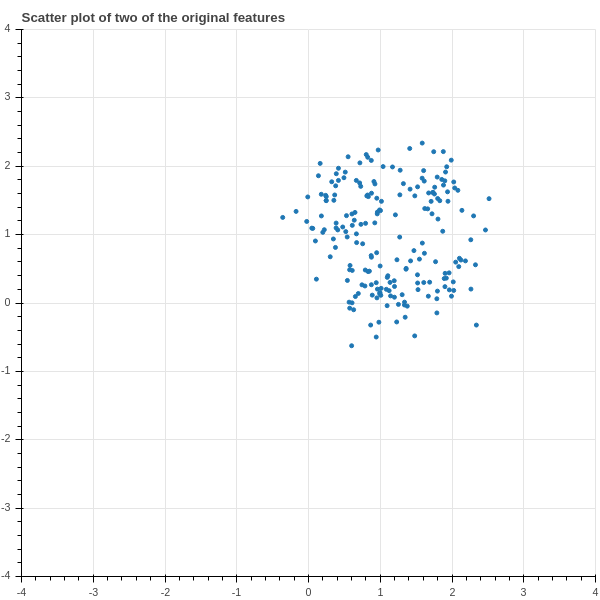
\includegraphics[width=0.5\textwidth,height=\textheight]{../img/features.png}
\caption{Scatter Plot of Two Features}\label{fig:features}
}
\end{figure}

Unfortunately there's not much to see in \cref{fig:features} -- just a
blob -- because the individual features of the data don't tell us much
in isolation, whatever structure there is in this data arises out of the
relationship between different features.

In \cref{fig:densitygrid} we show a ``density grid'' plot of the data.
The graph in position \(i,j\) shows a scatter plot of the \(i^{th}\) and
\(j^{th}\) columns of the data, except in the diagonal positions, where
in position \(i,i\) we plot a histogram of column \(i\). There's not
much structure visible; it is a lot of blobs.

\begin{figure}
\hypertarget{fig:densitygrid}{%
\centering
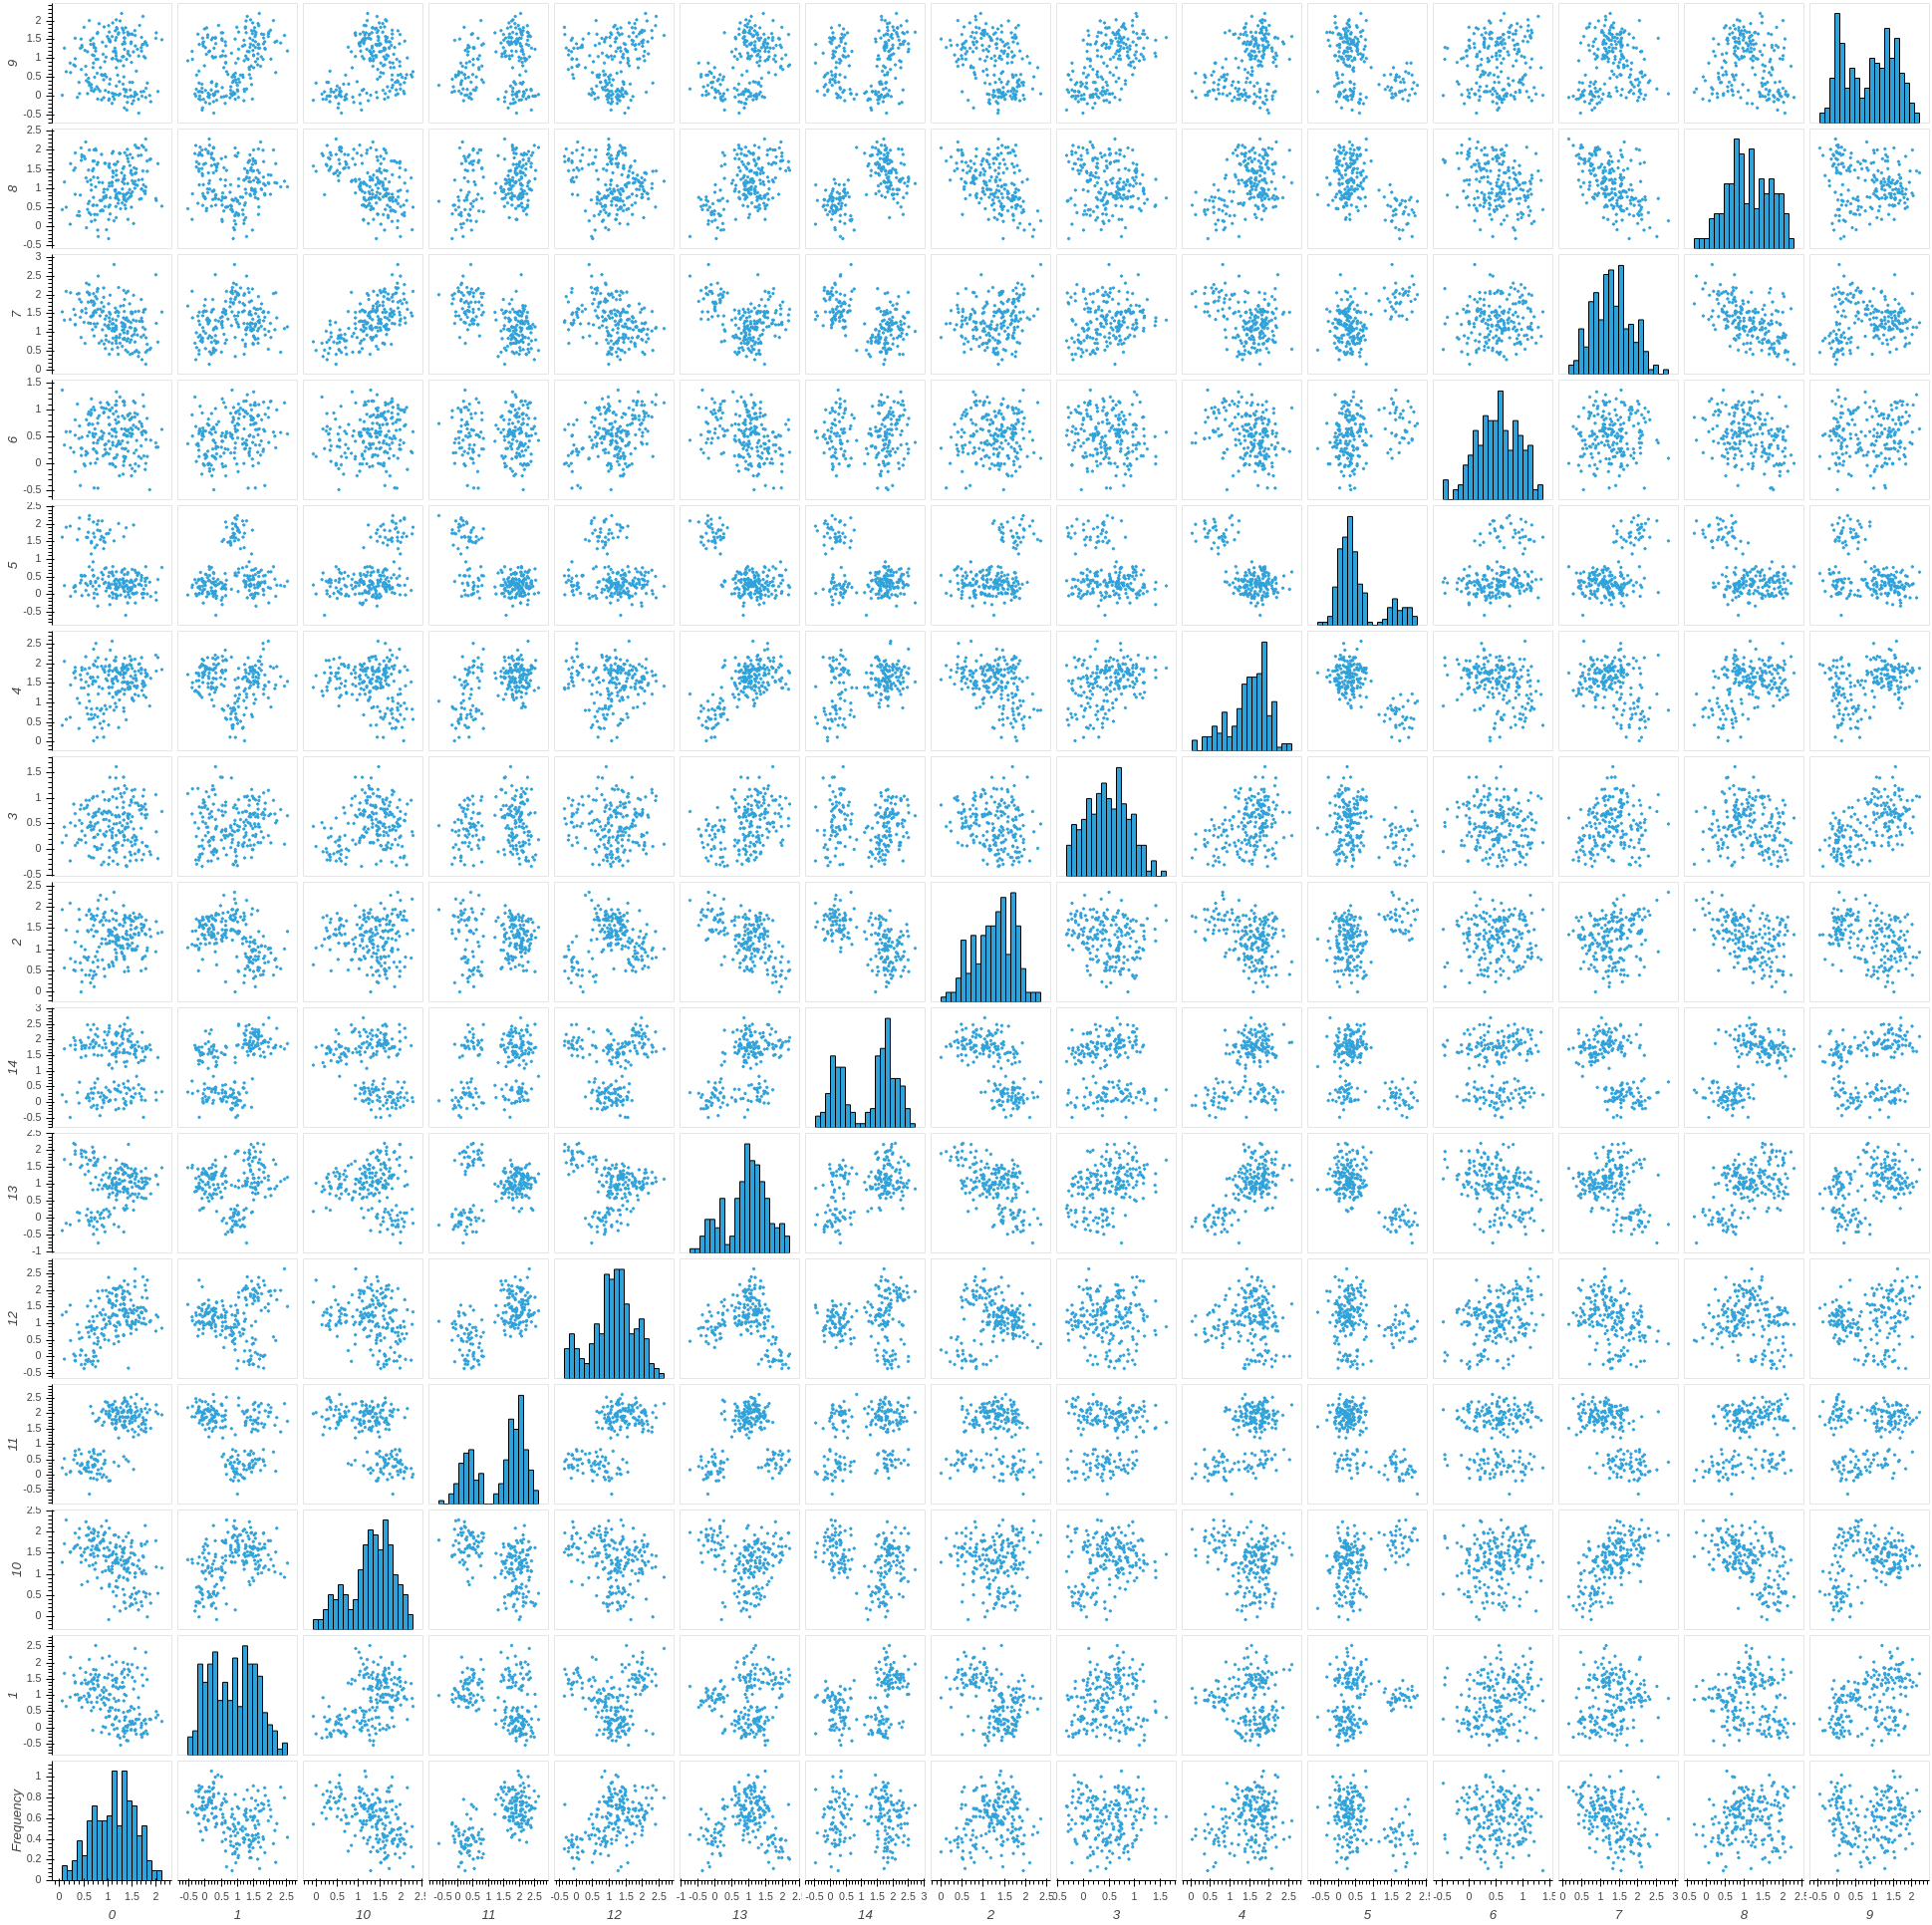
\includegraphics[width=0.5\textwidth,height=\textheight]{../img/density.png}
\caption{Density Grid Plot of All Features}\label{fig:densitygrid}
}
\end{figure}

So let's apply the theory of principal components. We use a software
package to compute the eigenvalues and eigenvectors of the matrix
\(D_{0}\). The \(15\) eigenvalues
\(\lambda_{1}\ge \cdots \ge \lambda_{15}\) are plotted, in descending
order, in \cref{fig:eigenvalues} .

\begin{figure}
\hypertarget{fig:eigenvalues}{%
\centering
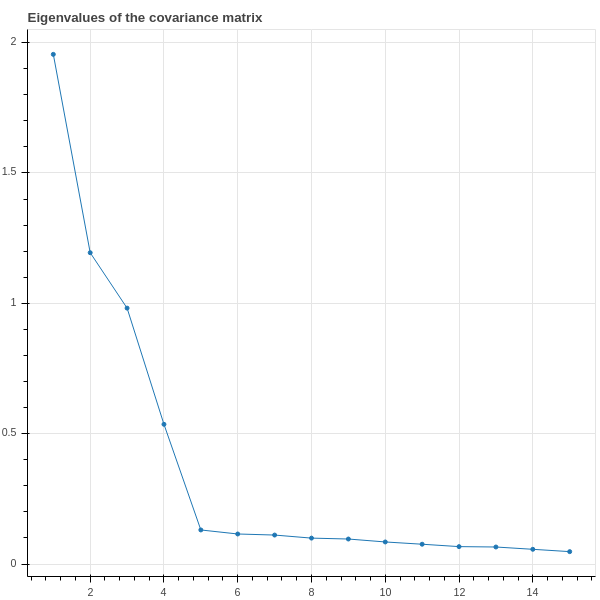
\includegraphics[width=0.5\textwidth,height=\textheight]{../img/eigenvalues.png}
\caption{Eigenvalues of the Covariance Matrix}\label{fig:eigenvalues}
}
\end{figure}

This plot shows that the first \(4\) eigenvalues are relatively large,
while the remaining \(11\) are smaller and not much different from each
other. We interpret this as saying that \emph{most of the variation in
the data is accounted for by the first four principal components.} We
can even make this quantitative. The \emph{total variance} of the data
is the sum of the eigenvalues of the covariance matrix -- the trace of
\(D_{0}\) -- and in this example that sum is around \(5\). The sum of
the first \(4\) eigenvalues is about \(4\), so the first four eignvalues
account for about \(4/5\) of the total variance, or about \(80\%\) of
the variation of the data.

Now let's focus in on the two largest eigenvalues \(\lambda_{1}\) and
\(\lambda_{2}\) and their corresponding eigenvectors \(u_{1}\) and
\(u_{2}\). The \(200\times 1\) column vectors \(S_{1}=X_{0}u_{1}\) and
\(S_{2}=X_{0}u_{2}\) are the values of the scores associated with these
two eigenvectors. So for each data point (each row of \(X_{0}\)) we have
two values (the corresponding entries of \(S_{1}\) and \(S_{2}\).) In
\cref{fig:principalvalues} we show a scatter plot of these scores.

\begin{figure}
\hypertarget{fig:principalvalues}{%
\centering
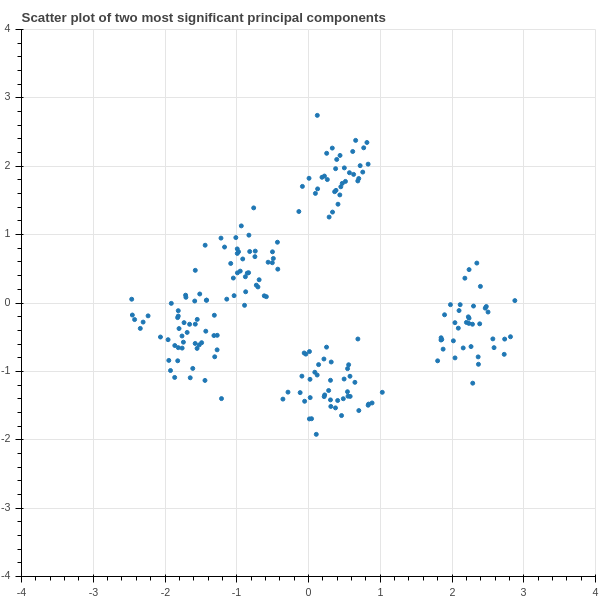
\includegraphics[width=0.5\textwidth,height=\textheight]{../img/pcadimred.png}
\caption{Scatter Plot of Scores in the First Two Principal
Directions}\label{fig:principalvalues}
}
\end{figure}

Notice that suddenly some structure emerges in our data! We can see that
the 200 points are separated into five clusters, distinguished by the
values of their scores! This ability to find hidden structure in
complicated data, is one of the most important applications of principal
components.

If we were dealing with real data, we would now want to investigate the
different groups of points to see if we can understand what
characteristics the principal components have identified.

\hypertarget{loadings}{%
\subsubsection{Loadings}\label{loadings}}

There's one last piece of the PCA puzzle that we are going to
investigate. In \cref{fig:principalvalues}, we plotted our data points
in the coordinates given by the first two principal components. In
geometric terms, we took the cloud of \(200\) points in
\(\mathbf{R}^{15}\) given by the rows of \(X_{0}\) and projected those
points into the two dimensional plane spanned by the eigenvectors
\(u_{1}\) and \(u_{2}\), and then plotted the distribution of the points
in that plane.

More generally, suppose we take our dataset \(X_{0}\) and consider the
first \(t\) principal components corresponding to the eigenvectors
\(u_{1},\ldots, u_{t}\). The projection of the data into the space
spanned by these eigenvectors is the represented by the
\(S = k\times t\) matrix \(X_{0}U\) where \(U\) is the \(N\times t\)
matrix whose columns are the eigenvectors \(u_{i}\). Each row of \(S\)
gives the values of the score arising from \(u_{i}\) in the \(i^{th}\)
column for \(i=1,\ldots, t\).

The remaining question that we wish to consider is: how can we see some
evidence of the original features in subspace? We can answer this by
imagining that we had an artificial sample \(x\) that has a measurement
of \(1\) for the \(i^{th}\) feature and a measurement of zero for all
the other features. The corresponding point is represented by a
\(1\times N\) row vector with a \(1\) in position \(i\). The projection
of this synthetic sample into the span of the first \(t\) principal
components is the \(1\times t\) vector \(xU\). Notice, however, that
\(xU\) is just the \(i^{th}\) row of the matrix \(U\). This vector in
the space spanned by the \(u_{i}\) is called the ``loading'' of the
\(i^{th}\) feature in the principal components.

This is illustrated in \cref{loadings}, which shows a line along the
direction of the loading corresponding to the each feature added to the
scatter plot of the data in the plane spanned by the first two principal
components. One observation one can make is that some of the features
are more ``left to right'', like features \(7\) and \(8\), while others
are more ``top to bottom'', like \(6\). So points that lie on the left
side of the plot have smaller values of features \(7\) and \(8\), while
those at the top of the plot have larger values of feature \(6\).

\begin{figure}
\hypertarget{fig:loadings}{%
\centering
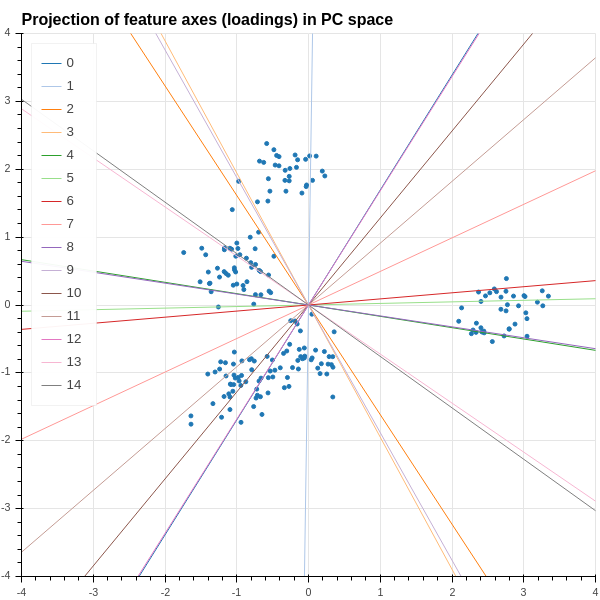
\includegraphics[width=0.5\textwidth,height=\textheight]{../img/loading.png}
\caption{Loadings in the Principal Component Plane}\label{fig:loadings}
}
\end{figure}

In the next, and last, section, of this discussion of Principal
Component Analysis, we will give proofs of the key mathematical ideas
summarized earlier in \cref{tbl:symmmat}, which have been central to
this analysis.

\hypertarget{sec:svd}{%
\subsubsection{The singular value decomposition}\label{sec:svd}}

The singular value decomposition is a slightly different way of looking
at principal components. Let \(\Lambda\) be the diagonal matrix of
eigenvalues of \(D_{0}\); we know that the entries of \(D_{0}\) are
non-negative. Let's drop the eigenvectors corresponding to the zero
eigenvalue. Let's say that there are \(s\) non-zero eigenvalues, and
\(s\) corresponding eigenvectors.

\textbf{Lemma:} Let \(P'\) be the \(N\times s\) matrix whose columns are
the eigenvectors with non-zero eigenvalues, and let \(\Lambda_{+}\) be
the \(s\times s\) diagonal matrix whose entries are the non-zero
eigenvalues. Then
\(P'\Lambda_{+} P'^{\intercal} = P\Lambda P^{\intercal} = D_{0}\).

\textbf{Proof:} First observe that \(P'\Lambda_{+}P'^{\intercal}\) is in
fact an \(N\times N\) matrix. Then look at the block structure to verify
the result.

The matrix \(\Lambda_{+}\) is diagonal, invertible, and, since the
eigenvalues are positive, it makes sense to consider the real matrix
\(\Lambda_{+}^{1/2}\) whose entries are the square roots of the
eigenvalues.

Let \(U = X_{0}P'\Lambda_{+}^{-1/2}\). Note that \(U\) is a
\(k\times s\) dimensional matrix.

\textbf{Lemma:} The columns of \(U\) are orthonormal.

\textbf{Proof:} Compute the \(s\times s\) matrix \(U^{\intercal}U\),
whose entries are all of the dot products of the columns of \(U\): \[
\begin{aligned}
U^{\intercal}U &=& \Lambda_{+}^{-1/2}P'^{\intercal}X_{0}^{\intercal}X_{0}P'\Lambda_{+}^{-1/2} \\
&=& \Lambda_{+}^{-1/2}P'^{\intercal}P'\Lambda_{+}P'^{\intercal}P'\Lambda_{+}^{-1/2} \\
&=& I_{s} \\
\end{aligned}
\] by the previous lemma and the fact that \(P'P'^{\intercal}\) is the
\(s\times s\) identity matrix.

Rearranging this yields the singular value decomposition.

\textbf{Theorem:} (The singular value decomposition) The matrix
\(X_{0}\) has a decomposition: \[
X_{0} = U\Lambda_{+}^{-1/2}P'^{\intercal}
\] where \(U\) (of dimension \(k\times s\)) and \(P'\) (of dimension
\(N\times s\)) are orthogonal, and \(\Lambda_{+}\) (of dimension
\(s\times s\)) is diagonal with positive entries. Furthermore, the
entries of \(\Lambda_{+}\) are the non-negative eigenvalues of
\(D_{0}=X_{0}^{\intercal}X_{0}\), and \(U\) and \(P'\) are uniquely
determined by \(X_{0}\).

\textbf{Proof:} We won't work through all of this, as it is a
reinterpretation of our work on principal components.

\textbf{Remark:} The entries of \(\Lambda_{+}^{-1/2}\) are called the
singular values of \(X_{0}\). They can be found directly by considering
the optimization problem implicitly equivalent to the problem we solved
in \cref{sec:subspaces}.

\hypertarget{sec:spectraltheorem}{%
\subsection{Eigenvalues and Eigenvectors of Real Symmetric Matrices (The
Spectral Theorem)}\label{sec:spectraltheorem}}

Now that we've shown how to apply the theory of eigenvalues and
eigenvectors of symmetric matrices to extract principal directions from
data, and to use those principal directions to find structure, we will
give a proof of the properties that we summarized in \cref{tbl:symmmat}.

A key tool in the proof is the Gram-Schmidt orthogonalization process.

\hypertarget{sec:gsprocess}{%
\subsubsection{Gram-Schmidt}\label{sec:gsprocess}}

\textbf{Proposition (Gram-Schmidt Process):} Let \(w_{1},\ldots, w_{k}\)
be a collection of linearly independent vectors in \(\mathbf{R}^{N}\)
and let \(W\) be the span of the \(w_{i}\). Let \(u_{1} = w_{1}\) and
let \[
u_{i} = w_{i} - \sum_{j=1}^{i-1} \frac{w_{i}\cdot u_{j}}{u_{j}\cdot u_{j}}u_{j}
\] for \(i=2,\ldots, k\). Then

\begin{itemize}
\tightlist
\item
  The vectors \(u_{i}\) are orthogonal: \(u_{i}\cdot u_{j}=0\) unless
  \(i=j\).
\item
  The vectors \(u_{i}\) span \(W\).
\item
  Each \(u_{i}\) is orthogonal to the all of \(w_{1},\ldots, w_{i-1}\).
\item
  The vectors \(u'_{i} = u_{i}/\|u_{i}\|\) are orthonormal.
\end{itemize}

\textbf{Proof:} This is an inductive exercise, and we leave it to you to
work out the details.

\hypertarget{the-spectral-theorem}{%
\subsubsection{The spectral theorem}\label{the-spectral-theorem}}

\textbf{Theorem:} Let \(D\) be a real symmetric \(N\times N\) matrix.
Then:

\begin{enumerate}
\def\labelenumi{\arabic{enumi}.}
\tightlist
\item
  All of the \(N\) eigenvalues
  \(\lambda_1\ge \lambda_2\ge \cdots \ge \lambda_{N}\) are real. If
  \(u^{\intercal}Du\ge 0\) for all \(u\in\mathbf{R}^{N}\), then all
  eigenvalues \(\lambda_{i}\ge 0\).
\item
  The matrix \(D\) is diagonalizable -- that is, it has \(N\) linearly
  independent eigenvectors.
\item
  If \(v\) and \(w\) are eigenvectors corresponding to eigenvalues
  \(\lambda\) and \(\lambda'\), with \(\lambda\not=\lambda'\), then
  \(v\) and \(w\) are orthogonal: \(v\cdot w=0\).
\item
  There is an orthonormal basis \(u_{1},\ldots, u_{N}\) of
  \(\mathbf{R}^{N}\) made up of eigenvectors for the eigenvalues
  \(\lambda_{i}\).
\item
  Let \(\Lambda\) be the diagonal matrix with entries
  \(\lambda_{1},\ldots, \lambda_{N}\) and let \(P\) be the matrix whose
  columns are made up of the eigenvectors \(u_{i}\). Then
  \(D=P\Lambda P^{\intercal}\).
\end{enumerate}

\textbf{Proof:} Start with \(1\). Suppose that \(\lambda\) is an
eigenvalue of \(D\). Let \(u\) be a corresponding nonzero eigenvector.
Then \(Du=\lambda u\) and
\(D\overline{u}=\overline{\lambda}\overline{u}\), where \(\overline{u}\)
is the vector whose entries are the conjugates of the entries of \(u\)
(and \(\overline{D}=D\) since \(D\) is real). Now we have \[
\overline{u}^{\intercal}Du = \lambda \overline{u}\cdot u = \lambda\|u\|^2
\] and \[
u^{\intercal}D\overline{u} = \overline{\lambda}u\cdot \overline{u} = \overline{\lambda}\|u\|^2.
\] But the left hand side of both of these equations are the same (take
the transpose and use the symmetry of \(D\)) so we must have
\(\lambda\|u\|^2 = \overline{\lambda}\|u\|^2\) so
\(\lambda=\overline{\lambda}\), meaning \(\lambda\) is real.

If we have the additional property that \(u^{\intercal}Du\ge 0\) for all
\(u\), then in particular
\(u_{i}^{\intercal}Du_{i} = \lambda\|u\|^2\ge 0\), and since
\(\|u\|^2> 0\) we must have \(\lambda\ge 0\).

Property \(2\) is in some ways the most critical fact. We know from the
general theory of the characteristic polynomial, and the fundamental
theorem of algebra, that \(D\) has \(N\) complex eigenvalues, although
some may be repeated. However, it may not be the case that \(D\) has
\(N\) linearly independent eigenvectors -- it may not be
\emph{diagonalizable}. So we will establish that now.

A one-by-one matrix is automatically symmetric and diagonalizable. In
the \(N\)-dimensional case, we know, at least, that \(D\) has at least
one eigenvector, and real one at that by part \(1\), and this gives us a
place to begin an inductive argument.

Let \(v_{N}\not=0\) be an eigenvector with eigenvalue \(\lambda\) and
normalized so that \(\|v_{N}\|^2=1\),\\
and extend this to a basis \(v_{1},\ldots v_{N}\) of \(\mathbf{R}^{N}\).
Apply the Gram-Schmidt process to construct an orthonormal basis of
\(\mathbf{R}^{N}\) \(u_{1},\ldots, u_{N}\) so that \(u_{N}=v_{N}\).

Any vector \(v\in\mathbf{R}^{N}\) is a linear combination \[
v = \sum_{i=1}^{N} a_{i}u_{i}
\] and, since the \(u_{i}\) are orthonormal, the coefficients can be
calculated as \(a_{i}=(u_{i}\cdot v)\).

Using this, we can find the matrix \(D'\) of the linear map defined by
our original matrix \(D\) in this new basis. By definition, if
\(d'_{ij}\) are the entries of \(D'\), then

\[
Du_{i} = \sum_{j=1}^{N} d'_{ij} u_{j}
\]

and so

\[
d'_{ij} = u_{j}\cdot Du_{i} = u_{j}^{\intercal}Du_{i}.
\]

Since \(D\) is symmetric,
\(u_{j}^{\intercal}Du_{i} =u_{i}^{\intercal}Du_{j}\) and so
\(d'_{ij}=d'_{ji}\). In other words, the matrix \(D'\) is still
symmetric. Furthermore,

\[
d'_{Ni} = u_{i}\cdot Du_{N} = u_{i}\cdot \lambda u_{N} = \lambda (u_{i}\cdot u_{N})
\]

since \(u_{N}=v_{N}\). Since the \(u_{i}\) are an orthonormal basis, we
see that \(d'_{iN}=0\) unless \(i=N\), and \(d'_{NN}=\lambda\).

In other words, the matrix \(D'\) has a block form: \[
D' = \left(\begin{matrix} * & * & \cdots &*  & 0 \\ \vdots & \vdots & \ddots   & \vdots & \vdots \\
* & * & \cdots &*  & 0 \\
0 & 0 & \cdots &0 &\lambda \end{matrix}\right)
\] and the block denoted by \(*\)'s is symmetric. If we call that block
\(D_{*}\), the inductive hypothesis tells us that the symmetric matrix
\(D_{*}\) is diagonalizable, so it has a basis of eigenvectors
\(u'_{1},\ldots, u'_{N-1}\) with eigenvalues
\(\lambda_{1},\ldots, \lambda_{N-1}\); this gives us a basis for the
subspace of \(\mathbf{R}^{N}\) spanned by \(u_{1},\ldots, u_{N-1}\)
which, together with \(u_{N}\) gives us a basis of \(\mathbf{R}^{N}\)
consisting of eigenvectors of \(D\).

This finishes the proof of Property \(2\).

For property \(3\), compute \[
v^{\intercal}Dw = \lambda'(v\cdot w)=w^{\intercal}Dv = \lambda (w\cdot v).
\] Since \(\lambda\not=\lambda'\), we must have \(v\cdot w=0\).

For property \(4\), if the eigenvalues are all distinct, this is a
consequence of property \(2\) -- you have \(N\) eigenvectors, scaled to
length \(1\), for different eigenvalues, and by \(2\) they are
orthogonal. So the only complication is the case where some eigenvalues
are repeated. If \(\lambda\) occurs \(r\) times, then you have \(r\)
linearly independent vectors \(u_{1},\ldots, u_{r}\) that span the
\(\lambda\) eigenspace. The Gram-Schmidt process allows you to construct
an orthonormal set that spans this eigenspace, and while this
orthonormal set isn't unique, any one of them will do.

For property \(5\), let \(e_{i}\) be the column vector that is zero
except for a \(1\) in position \(i\). The product
\(e_{j}^{\intercal}De_{i}=d_{ij}\). Let's write \(e_{i}\) and \(e_{j}\)
in terms of the orthonormal basis \(u_{1},\ldots u_{N}\): \[
e_{i} = \sum_{k=1}^{N} (e_{i}\cdot u_{k})u_k \hbox{ and } e_{j} = \sum_{k=1}^{N}(e_{j}\cdot u_{k})u_{k}.
\] Using this expansion, we compute \(e_{j}^{\intercal}De_{i}\) in a
more complicated way: \[
e_{j}^{\intercal}De_{i} = \sum_{r=1}^{N}\sum_{s=1}^{N} (e_{j}\cdot u_{r})(e_{i}\cdot u_{s})(u_{r}^{\intercal}Du_{s}).
\] But \(u_{r}^{\intercal}Du_{s}=\lambda_{s}(u_{r}\cdot u_{s})=0\)
unless \(r=s\), in which case it equals \(\lambda_{r}\), so \[
e_{j}^{\intercal}De_{i} = \sum_{r=1}^{N} \lambda_{r}(e_{j}\cdot u_{r})(e_{i}\cdot u_{r}).
\] On the other hand, \[
P^{\intercal}e_{i} = \left[\begin{matrix} (e_{i}\cdot u_{1})\\ (e_{i}\cdot u_{2})\\ \vdots \\(e_{i}\cdot u_{N})\end{matrix}\right]
\] and \[
\Lambda P^{\intercal}e_{i} = \left[\begin{matrix} \lambda_{1}(e_{i}\cdot u_{i})\\ \lambda_{2}(e_{i}\cdot u_{2})\\ \vdots \\ \lambda_{N}(e_{i}\cdot u_{N})\end{matrix}\right]
\] Therefore the \(i,j\) entry of \(P\Lambda P^{\intercal}\) is \[
(e_{j}^{\intercal}P)\Lambda (P^{\intercal}e_{j}) = \sum_{r=1}^{N} \lambda_{r}(e_{i}\cdot u_{r})(e_{j}\cdot u_{r}) = d_{ij}
\] so the two matrices \(D\) and \(P\Lambda P^{\intercal}\) are in fact
equal.

\textbf{Exercises:}

\begin{enumerate}
\def\labelenumi{\arabic{enumi}.}
\item
  Prove the rest of the first lemma in \cref{sec:svd}.
\item
  Prove the Gram-Schmidt Process has the claimed properties in
  \cref{sec:gsprocess}.
\end{enumerate}

\end{document}
